\documentclass[tikz,border=10pt]{standalone}
% Shared look for every TikZ diagram. Load with % Shared look for every TikZ diagram. Load with % Shared look for every TikZ diagram. Load with \input{../../tools/tikz-style.tex}
\usepackage[T1]{fontenc}
\usepackage{lmodern}
\renewcommand{\sfdefault}{lmr}  % diagrams use the same serif as the text
\usetikzlibrary{arrows.meta, positioning, shapes.geometric, calc, fit, backgrounds}
\definecolor{cblue}{HTML}{4C78A8}
\definecolor{corange}{HTML}{F58518}
\definecolor{cgreen}{HTML}{54A24B}
\definecolor{cred}{HTML}{E45756}
\definecolor{cpurple}{HTML}{B279A2}
\definecolor{cgrey}{HTML}{6B6B6B}
\tikzset{
  every picture/.style={font=\sffamily, line width=1.2pt},
  box/.style={draw=#1, fill=#1!12, rounded corners=4pt, align=center, inner sep=7pt, minimum height=1.1cm},
  box/.default=cgrey,
  arrow/.style={-{Stealth[length=3mm]}, draw=cgrey, line width=1.4pt},
  title/.style={font=\sffamily\bfseries\Large},
  note/.style={font=\sffamily\small, text=cgrey, align=center},
}
\AtBeginDocument{\hyphenpenalty=10000 \exhyphenpenalty=10000}

\usepackage[T1]{fontenc}
\usepackage{lmodern}
\renewcommand{\sfdefault}{lmr}  % diagrams use the same serif as the text
\usetikzlibrary{arrows.meta, positioning, shapes.geometric, calc, fit, backgrounds}
\definecolor{cblue}{HTML}{4C78A8}
\definecolor{corange}{HTML}{F58518}
\definecolor{cgreen}{HTML}{54A24B}
\definecolor{cred}{HTML}{E45756}
\definecolor{cpurple}{HTML}{B279A2}
\definecolor{cgrey}{HTML}{6B6B6B}
\tikzset{
  every picture/.style={font=\sffamily, line width=1.2pt},
  box/.style={draw=#1, fill=#1!12, rounded corners=4pt, align=center, inner sep=7pt, minimum height=1.1cm},
  box/.default=cgrey,
  arrow/.style={-{Stealth[length=3mm]}, draw=cgrey, line width=1.4pt},
  title/.style={font=\sffamily\bfseries\Large},
  note/.style={font=\sffamily\small, text=cgrey, align=center},
}
\AtBeginDocument{\hyphenpenalty=10000 \exhyphenpenalty=10000}

\usepackage[T1]{fontenc}
\usepackage{lmodern}
\renewcommand{\sfdefault}{lmr}  % diagrams use the same serif as the text
\usetikzlibrary{arrows.meta, positioning, shapes.geometric, calc, fit, backgrounds}
\definecolor{cblue}{HTML}{4C78A8}
\definecolor{corange}{HTML}{F58518}
\definecolor{cgreen}{HTML}{54A24B}
\definecolor{cred}{HTML}{E45756}
\definecolor{cpurple}{HTML}{B279A2}
\definecolor{cgrey}{HTML}{6B6B6B}
\tikzset{
  every picture/.style={font=\sffamily, line width=1.2pt},
  box/.style={draw=#1, fill=#1!12, rounded corners=4pt, align=center, inner sep=7pt, minimum height=1.1cm},
  box/.default=cgrey,
  arrow/.style={-{Stealth[length=3mm]}, draw=cgrey, line width=1.4pt},
  title/.style={font=\sffamily\bfseries\Large},
  note/.style={font=\sffamily\small, text=cgrey, align=center},
}
\AtBeginDocument{\hyphenpenalty=10000 \exhyphenpenalty=10000}

\begin{document}
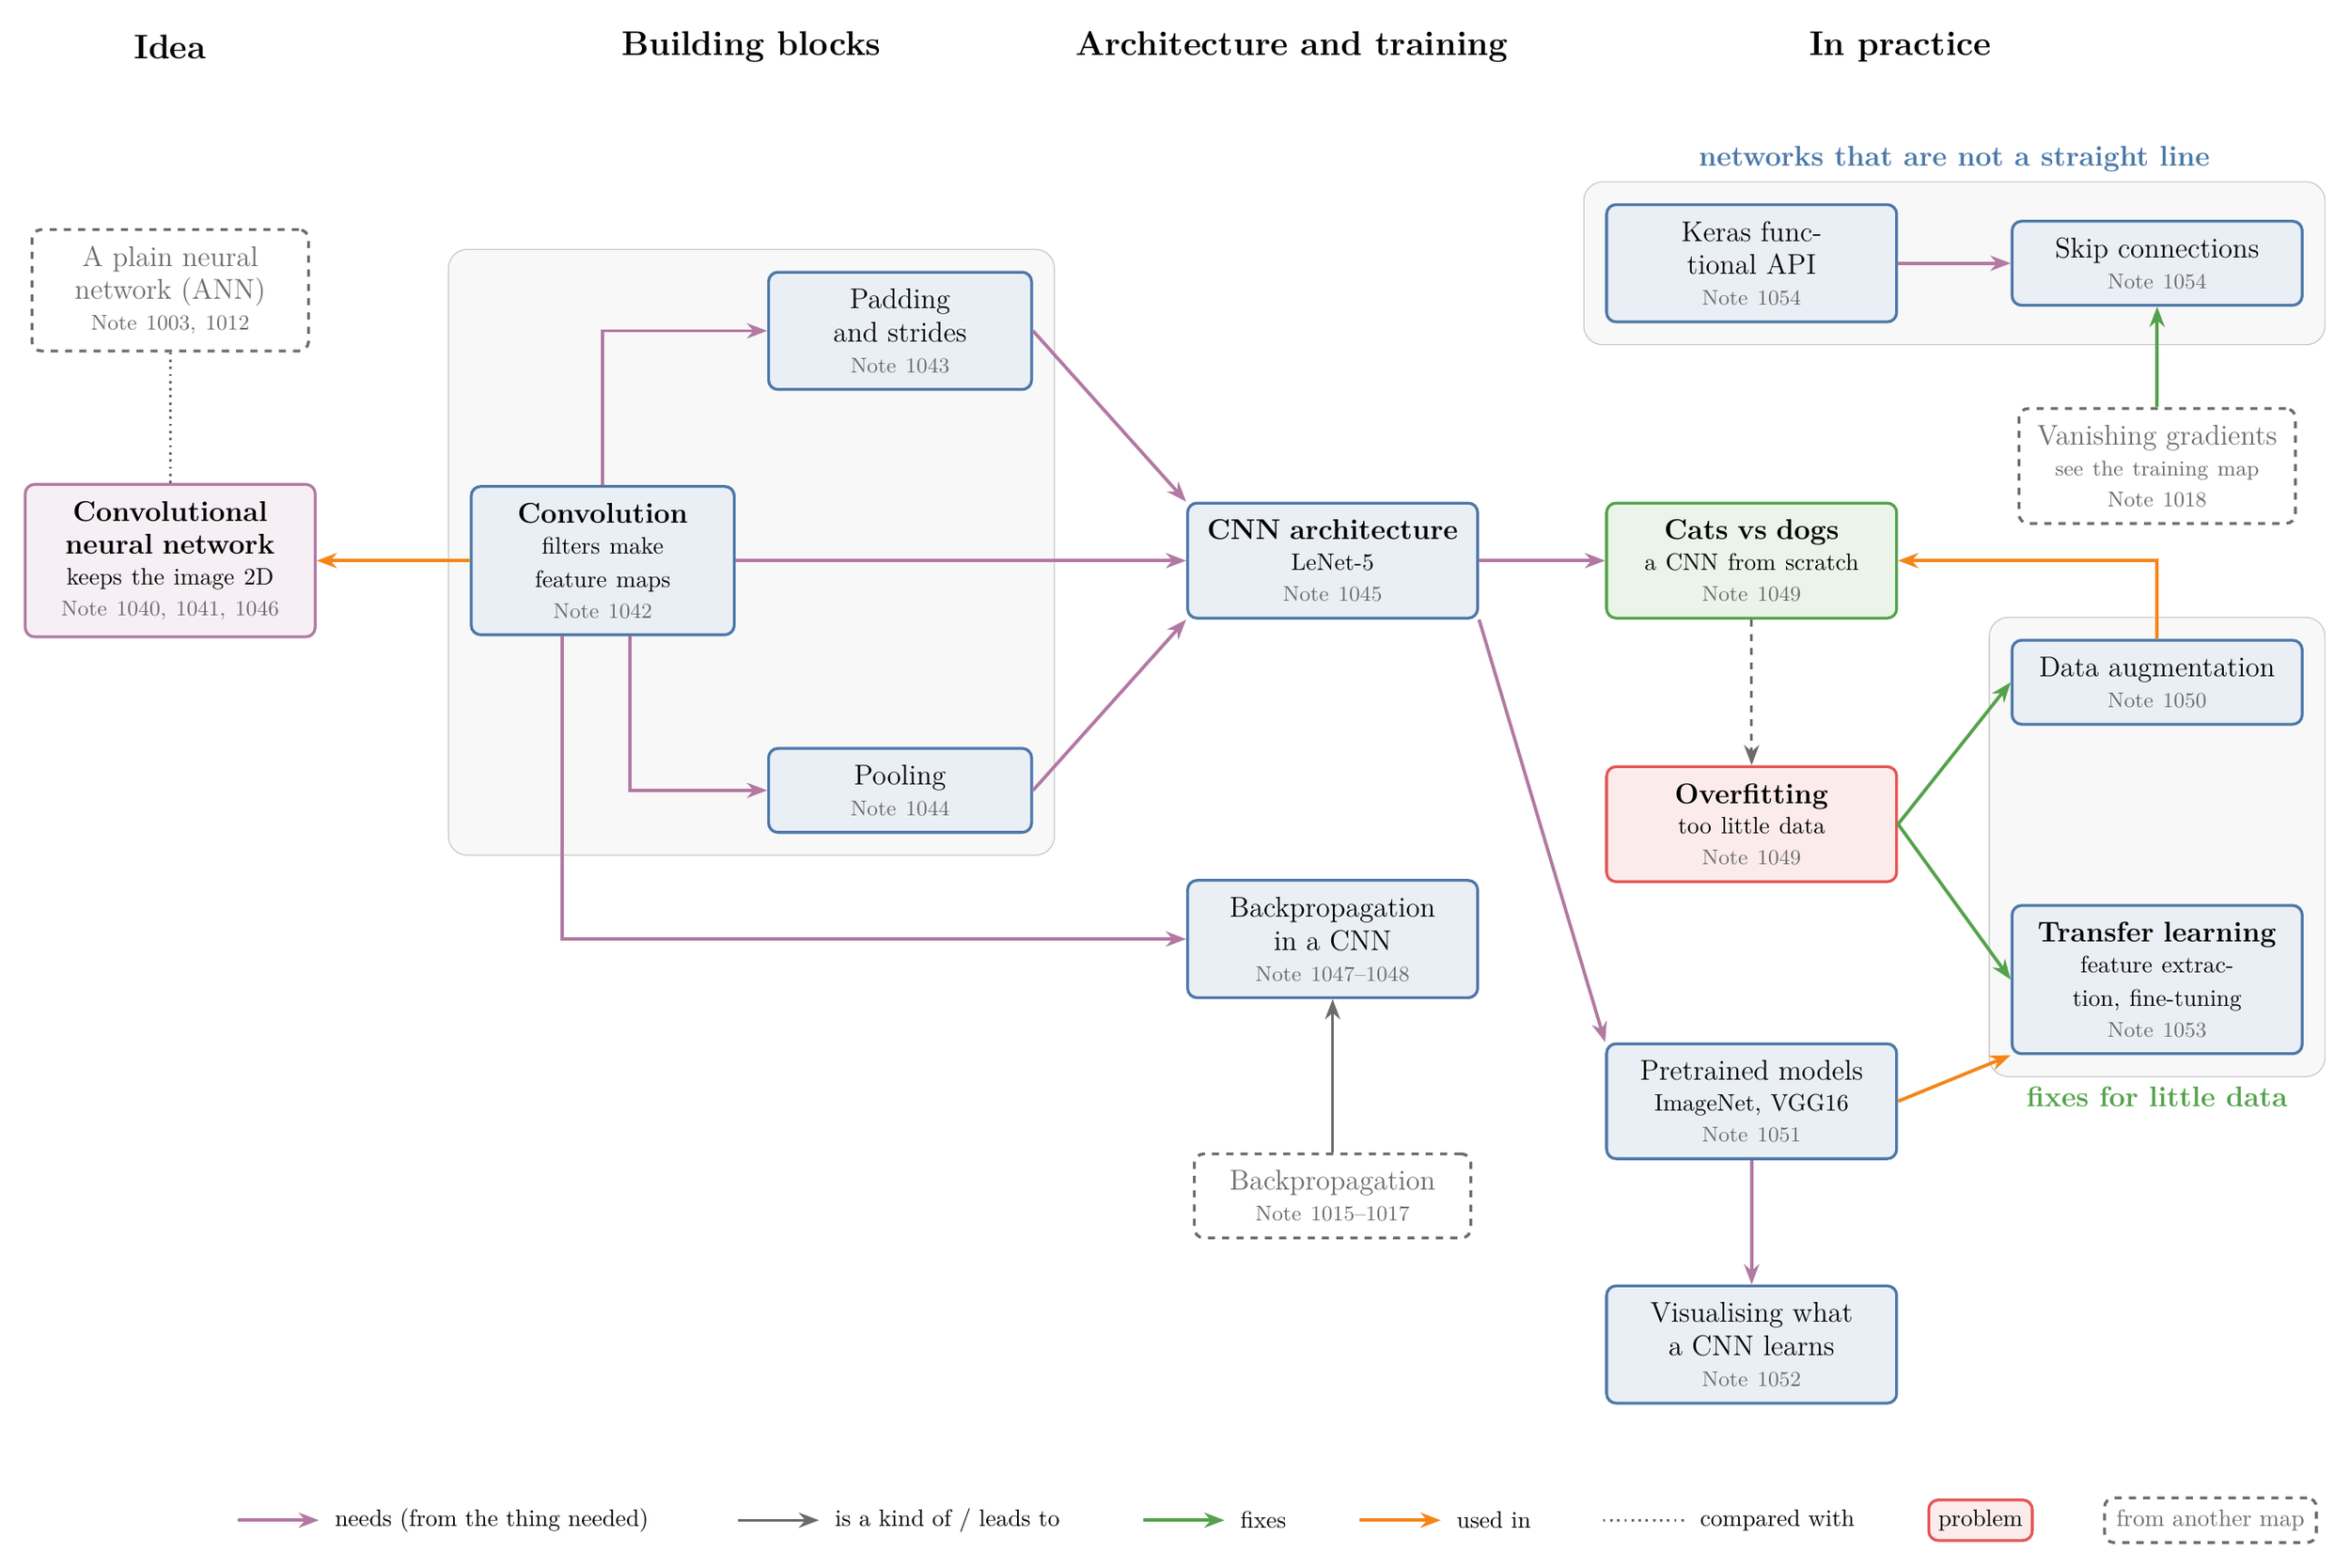
\begin{tikzpicture}[
    every node/.append style={font=\sffamily\large},
    con/.style={box=cblue, text width=3.8cm},
    prob/.style={box=cred, text width=3.8cm},
    goal/.style={box=cgreen, text width=3.8cm},
    prev/.style={draw=cgrey, dashed, rounded corners=4pt, align=center, inner sep=7pt, text=cgrey, text width=3.6cm, minimum height=1.1cm},
    group/.style={draw=cgrey!40, fill=cgrey!5, rounded corners=8pt, inner sep=9pt},
    kind/.style={arrow, draw=cgrey, line width=1pt},
    needs/.style={arrow, draw=cpurple},
    fixes/.style={arrow, draw=cgreen},
    usedin/.style={arrow, draw=corange},
    cmp/.style={draw=cgrey, line width=1pt, dotted},
  ]
  \newcommand{\nt}[1]{\\[-1pt]{\small\color{cgrey}Note #1}}
  \newcommand{\sub}[1]{\\[-1pt]{\normalsize #1}}
  \node[title] at (0,10.6) {Idea};
  \node[title] at (8.6,10.6) {Building blocks};
  \node[title] at (16.6,10.6) {Architecture and training};
  \node[title] at (25.6,10.6) {In practice};

  % idea
  \node[prev] (ann) at (0,7.0) {A plain neural network (ANN)\nt{1003, 1012}};
  \node[box=cpurple, text width=3.8cm, minimum height=2.2cm] (cnn) at (0,3) {\textbf{Convolutional neural network}\sub{keeps the image 2D}\nt{1040, 1041, 1046}};
  \draw[cmp] (ann) -- (cnn);

  % building blocks
  \node[con, text width=3.4cm] (conv) at (6.4,3) {\textbf{Convolution}\sub{filters make feature maps}\nt{1042}};
  \node[con, text width=3.4cm] (pad)  at (10.8,6.4) {Padding and strides\nt{1043}};
  \node[con, text width=3.4cm] (pool) at (10.8,-0.4) {Pooling\nt{1044}};
  \begin{scope}[on background layer]
    \node[group, fit=(conv) (pad) (pool)] (gb) {};
  \end{scope}

  % architecture and training
  \node[con] (lenet) at (17.2,3) {\textbf{CNN architecture}\sub{LeNet-5}\nt{1045}};
  \node[con] (cbp)   at (17.2,-2.6) {Backpropagation in a CNN\nt{1047--1048}};
  \node[prev] (bp)   at (17.2,-6.4) {Backpropagation\nt{1015--1017}};

  % in practice
  \node[box=cgreen, text width=3.8cm] (proj) at (23.4,3) {\textbf{Cats vs dogs}\sub{a CNN from scratch}\nt{1049}};
  \node[prob] (over) at (23.4,-0.9) {\textbf{Overfitting}\sub{too little data}\nt{1049}};
  \node[con] (aug)   at (29.4,1.2) {Data augmentation\nt{1050}};
  \node[con] (tl)    at (29.4,-3.2) {\textbf{Transfer learning}\sub{feature extraction, fine-tuning}\nt{1053}};
  \node[con] (pre)   at (23.4,-5.0) {Pretrained models\sub{ImageNet, VGG16}\nt{1051}};
  \node[con] (vis)   at (23.4,-8.6) {Visualising what a CNN learns\nt{1052}};
  \node[con] (fapi)  at (23.4,7.4) {Keras functional API\nt{1054}};
  \node[con] (skip)  at (29.4,7.4) {Skip connections\nt{1054}};
  \node[prev] (van)  at (29.4,4.4) {Vanishing gradients\\[-1pt]{\small see the training map}\nt{1018}};
  \begin{scope}[on background layer]
    \node[group, fit=(aug) (tl)] (gf) {};
    \node[group, fit=(fapi) (skip)] (gn) {};
  \end{scope}
  \node[font=\sffamily\bfseries\large, text=cgreen, anchor=north] at (gf.south) {fixes for little data};
  \node[font=\sffamily\bfseries\large, text=cblue, anchor=south] at (gn.north) {networks that are not a straight line};

  % links
  \draw[usedin] (conv.west) -- (cnn.east);
  \draw[needs] (conv.north) |- (pad.west);
  \draw[needs] ([xshift=0.4cm]conv.south) |- (pool.west);
  \draw[needs] (conv.east) -- (lenet.west);
  \draw[needs] (pad.east) -- (lenet.north west);
  \draw[needs] (pool.east) -- (lenet.south west);
  \draw[needs] ([xshift=-0.6cm]conv.south) |- (cbp.west);
  \draw[kind] (bp) -- (cbp);
  \draw[needs] (lenet.east) -- (proj.west);
  \draw[needs] (lenet.south east) -- (pre.north west);
  \draw[kind, dashed] (proj) -- (over);
  \draw[fixes] (over.east) -- (aug.west);
  \draw[fixes] (over.east) -- (tl.west);
  \draw[usedin] (aug.north) |- (proj.east);
  \draw[usedin] (pre.east) -- (tl.south west);
  \draw[needs] (pre) -- (vis);
  \draw[needs] (fapi) -- (skip);
  \draw[fixes] (van) -- (skip);

  % legend
  \begin{scope}[shift={(1.0,-11.2)}, every node/.style={font=\sffamily, anchor=west}]
    \draw[needs] (0,0) -- (1.2,0);      \node at (1.3,0) {needs (from the thing needed)};
    \draw[kind] (7.4,0) -- (8.6,0);     \node at (8.7,0) {is a kind of / leads to};
    \draw[fixes] (13.4,0) -- (14.6,0);  \node at (14.7,0) {fixes};
    \draw[usedin] (16.6,0) -- (17.8,0); \node at (17.9,0) {used in};
    \draw[cmp] (20.2,0) -- (21.4,0);    \node at (21.5,0) {compared with};
    \node[box=cred, minimum height=0.6cm, inner sep=4pt, anchor=west] at (25.0,0) {problem};
    \node[draw=cgrey, dashed, rounded corners=4pt, inner sep=5pt, text=cgrey, anchor=west] at (27.6,0) {from another map};
  \end{scope}
\end{tikzpicture}
\end{document}
